\documentclass[pdf]{beamer}
\mode<presentation>{} 

\usepackage{enumitem}
\usepackage{graphicx}
\usepackage{bbding}
\usepackage{pifont}
\usepackage{hyperref}
\usepackage{pgf}
\usepackage{tikz}
\usepackage{tikz-qtree,tikz-qtree-compat}
\usetikzlibrary{trees}
\usetikzlibrary{arrows,automata}
\usetikzlibrary{automata,positioning}
\usetikzlibrary{shapes}
\usepackage{pgfornament}
\usepackage{eso-pic}
\usepackage[absolute,overlay]{textpos}
\usepackage[scaled=1]{helvet}
\usepackage{times}
\usepackage{courier}
\usepackage{rotunda}
\usepackage{mathtools,enumerate,amssymb}
\usepackage[utf8]{inputenc}
\usepackage[T1]{fontenc}
\usepackage{color}
\usepackage{overpic}
\usepackage{minibox}
\usetikzlibrary{patterns}
\usepackage[utf8]{inputenc}
\usepackage[T1]{fontenc}
\usepackage{graphicx}
\usepackage{varwidth}
\usepackage{xcolor}
\usepackage{multicol}
\usepackage{multirow}
\usepackage[export]{adjustbox}
\usepackage{wrapfig}
\usepackage{textcomp}
\usepackage[export]{adjustbox}
\usepackage{longtable}



\definecolor{background}{RGB}{255,255,255}
\setbeamercolor{background canvas}{bg=background}
\setbeamercolor{frametitle}{fg=blue}



\title{Design guidelines and usability heuristics}
\subtitle{Human Computer Interaction}
\AtBeginSection[]{}



\setbeamertemplate{sidebar right}{}
\setbeamertemplate{footline}{%
\hfill\usebeamertemplate***{navigation symbols}
\hspace{1cm}\insertframenumber{}/\inserttotalframenumber}

\graphicspath{{./img/}}



\begin{document}



{\setbeamercolor{background canvas}{bg=background}
\begin{frame}
\vspace{10mm}
\huge{\raggedleft{\color{black}{\textbf{Design guidelines and usability heuristics}}}}

\large{\raggedleft{\color{black} Human Computer Interaction}}

\begin{flushright}
\end{flushright}

\fontsize{7pt}{1pt}\selectfont{
Based on slide deck 

\textbf{Part 5: Principles for Design. Design guidelines and usability heuristics}

Human Computer Interaction I: Principles and Design

by

\textbf{Saul Greenberg}
\newline
Professor
\newline
\textbf{University of Calgary, Canada}

\textit{The new slides are marked with a *}
}

\fontsize{5pt}{1pt}\selectfont{ \textcolor{lightgray}
{Slide deck by Saul Greenberg. Permission is granted to use this for non-commercial purposes as long as general credit to Saul Greenberg is clearly maintained.
Warning: some material in this deck is used from other sources without permission. Credit to the original source is given if it is known.}}

\end{frame}}



% Inaintea codului fiecarui slide se vor scrie urmatoarele informatii:
% Nume si prenume student
% Numarul slide-ului corespunzator din prezentarea prof. Saul Greenberg
% Numele imaginilor inserate trebuie sa fie numar_slide_nume_imagine.extensie_imagine

%Sava Mircea
%Numarul slide-ului: 1
\begin{frame}
	\textbf{\LARGE Usability Heuristics \LARGE}
   	\bigskip
    \\
    {- Avoid common design pitfalls by following 9 design principles}
    \bigskip
    \\
    {- Inspect an interface for usability problems with these principles}
    \newline
    \newline
    \newline
   	\textbf{\LARGE Evaluating Heuristic evaluation \LARGE}
    \newline
    \newline
    \newline
   	\textbf{\LARGE Style guides \LARGE}
\end{frame}



%Sava Mircea
%Numarul slide-ului: 2
\begin{frame}
{\textbf{Design principles}}{\textcolor{red}{\rule{12cm}{1.2pt}}}

\textbf{broad usability statements that guide a developer's design efforts}
    \\
    \begin{itemize}
    	\item[--] use the users language
        \item[--] provide feedback ...
    \end{itemize}
    \bigskip
\textbf{derived from common design problems across many systems}
    \vspace{100px}
\end{frame}



%Sava Mircea
%Numarul slide-ului: 3
\begin{frame}
{\textbf{Heuristic evaluation}}{\textcolor{red}{\rule{12cm}{1.2pt}}}

    \textbf{Systematic inspection to see if interface complies to guidelines}
    \bigskip
    \\
    \textbf{Method}
    \begin{itemize}
    	\item[--] 3-5 inspectors
        \item[--] usability engineers, end users, double experts ...
        \item[--] inspect interface in isolation (approx. 1-2 hours for simple interfaces)
        \item[--] compare notes afterwards
        \begin{itemize}
        	\item[\textcolor{black}{•}] single evaluator only catches around 35\% of usability problems
            \item[\textcolor{black}{•}] 5 evaluators catch around 75\%
        \end{itemize}
    \end{itemize}
    \bigskip
    \textbf{Works for paper, prototypes, and working systems}
    \vspace{40px}

\end{frame}



%Sava Mircea
%Numarul slide-ului: 4
\begin{frame}
{\textbf{Heuristic evaluation}}{\textcolor{red}{\rule{12cm}{1.2pt}}}

    \textbf{Advantages}
    \begin{itemize}
    	\item[--] "minimalist" approach
        \begin{itemize}
        	\item[\textcolor{black}{•}] a few guidelines identify many common usability problems
            \item[\textcolor{black}{•}] easily remembered
            \item[\textcolor{black}{•}] easily applied with modest effort
        \end{itemize}
        \bigskip
        \item[--] discount usability engineering
        \begin{itemize}
        	\item[\textcolor{black}{•}] end users not required
            \item[\textcolor{black}{•}] cheap and fast way to inspect a system
            \item[\textcolor{black}{•}] can be done by usability experts, double experts, and end users
        \end{itemize}
    \end{itemize}
    \vspace{20px}
\end{frame}



\begin{frame}
{\textbf{Heuristic evaluation}}{\textcolor{red}{\rule{12cm}{1.2pt}}}

    \textbf{Problems}
    \begin{itemize}
    	\item[--] principles are more or less at the motherhood level
        \begin{itemize}
        	\item[\textcolor{black}{•}] can't be treated as a simple check-list
            \item[\textcolor{black}{•}] subtleties involved in their use
        \end{itemize}
    \end{itemize}
    \vspace{20px}
\end{frame}



%Sava Mircea
%Numarul slide-ului: 5
%5_picture1.png
%5_picture2.png
%5_picture3.png
\begin{frame}
{\textbf{1. Simple and natural dialogue}}{\textcolor{red}{\rule{12cm}{1.2pt}}}

    \bigskip
    \begin{itemize}
    	\item[--] use the user's conceptual model
        \item[--] match user's task sequence
        \item[--] minimize mapping between interface and task semantics
    \end{itemize}
    \bigskip
    \begin{picture}(0,0)
      \put(5,-30){\hbox{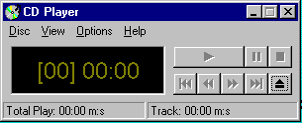
\includegraphics[scale=0.43]{5_picture1.png}}}
  	\end{picture}
    \begin{picture}(0,0)
      \put(120,-115){\hbox{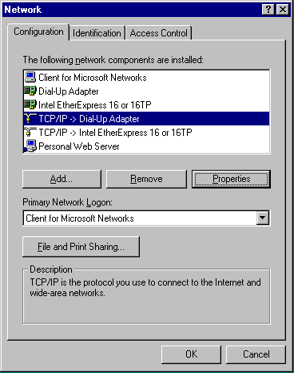
\includegraphics[scale=0.45]{5_picture2.png}}}
  	\end{picture}
    \begin{picture}(0,0)
      \put(170,-129){\hbox{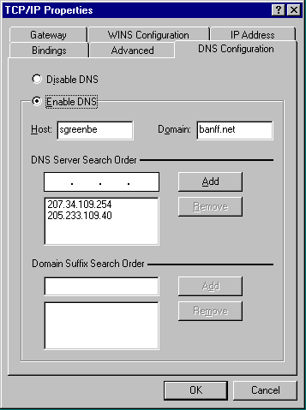
\includegraphics[scale=0.45]{5_picture3.png}}}
  	\end{picture}
    \vspace{160px}
\end{frame}



%Sava Mircea
%Numarul slide-ului: 6
\begin{frame}
{\textbf{1. Simple and natural dialogue}}{\textcolor{red}{\rule{12cm}{1.2pt}}}

    \textbf{Present exactly the information the user needs}
    \begin{itemize}
    	\item[--] less is more 
        \begin{itemize}
        	 \item[\textcolor{black}{•}] less to learn, to get wrong, to distract ...
        \end{itemize}
        \bigskip
        \item[--] information should appear in natural order
        \begin{itemize}
        	\item[\textcolor{black}{•}] related information is graphically clustered
            \item[\textcolor{black}{•}] order of accessing information matches user's 									      expectations
        \end{itemize}
        \bigskip
        \item[--] remove or hide irrelevant or rarely needed information
        \begin{itemize}
         	\item[\textcolor{black}{•}] competes with important information on screen
        \end{itemize}
        \bigskip
        \item[--] remove modes
        \bigskip
        \item[--] use windows frugally
        \begin{itemize}
         	\item[\textcolor{black}{•}] don't add unneeded navigation and windows management
        \end{itemize}
    \end{itemize}
  
\end{frame}



%Sava Mircea
%Numarul slide-ului: 7
%7_picture1.png
\begin{frame}
{\textbf{1. Simple and natural dialogue}}{\textcolor{red}{\rule{12cm}{1.2pt}}}

    \begin{picture}(0,0)
      \put(42,-110){\hbox{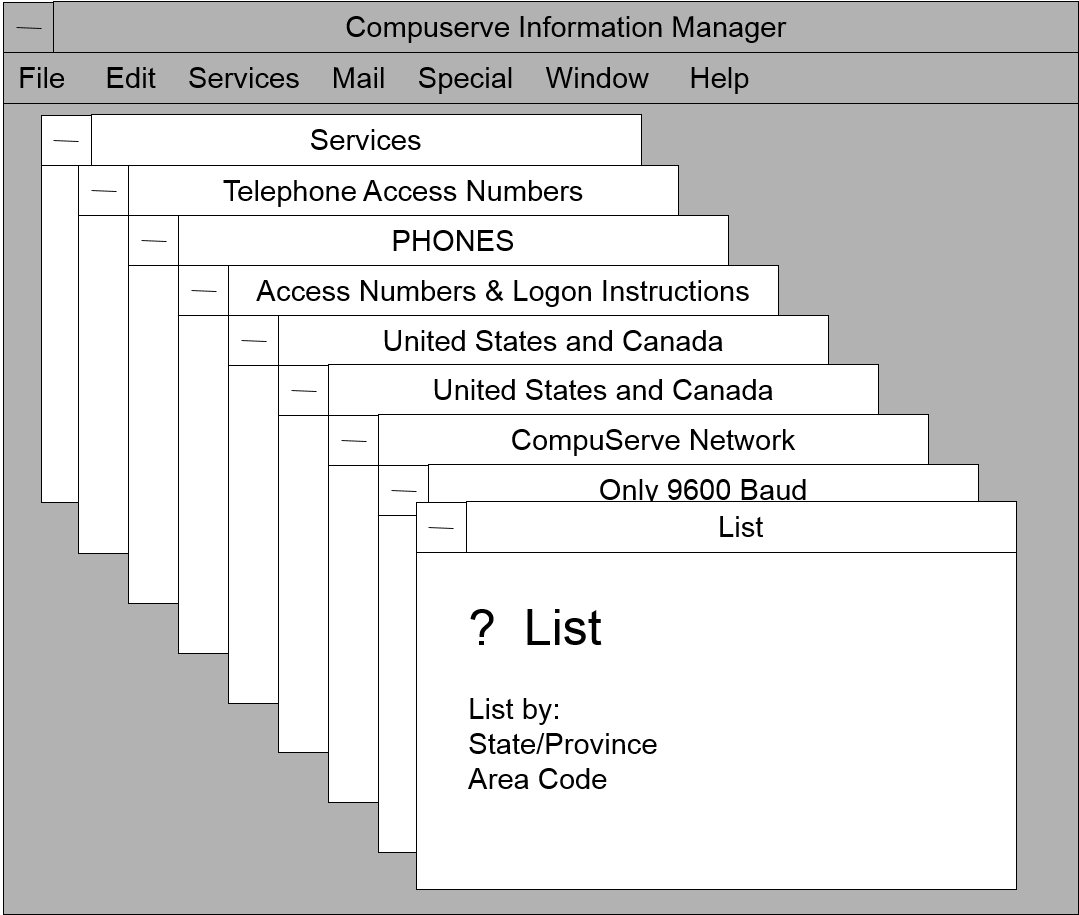
\includegraphics[scale=0.47]{7_picture1.png}}}
  	\end{picture}
  	
\end{frame}



%Sava Mircea
%Numarul slide-ului: 8
%8_picture1.png
\begin{frame}
{\textbf{1. Simple and natural dialogue}}{\textcolor{red}{\rule{12cm}{1.2pt}}}

	\begin{figure}[b]
      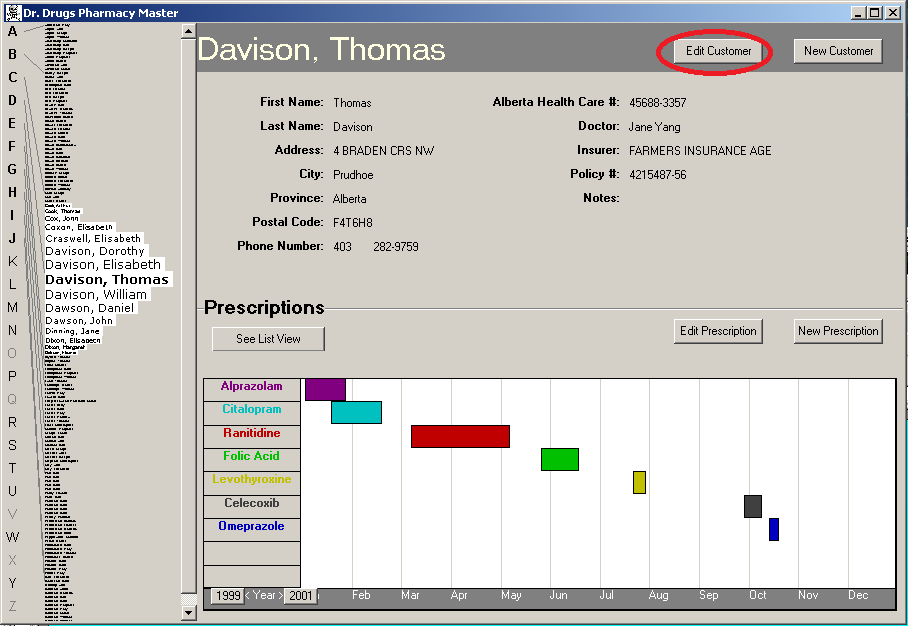
\includegraphics[scale = 0.47]{8_picture1.png}
  	\end{figure}
    \hspace{150px}\fontsize{7pt}{10pt}\textbf{Good: Information all in the same place}
   
    \fontsize{4pt}{1pt}\selectfont{\color{gray}By previous 481 students Brant LeClercq, Lloyd Yoon, Amy Yang (with permission)}
 
\end{frame}



%Tica Alexandru
%nr slide 9
\begin{frame}
{\textbf{1. Simple and natural dialogue}}{\textcolor{red}{\rule{12cm}{1.2pt}}}

	\begin{figure}[b]
      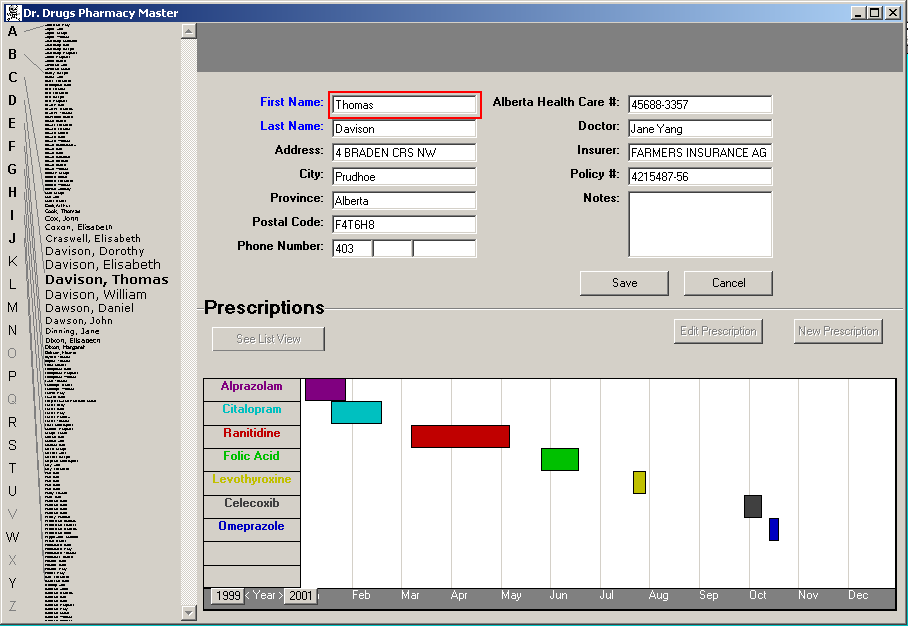
\includegraphics[scale = 0.47]{9_Picture1.png}
  	\end{figure}

    \hspace{150px}\fontsize{7pt}{10pt}\textbf{Good: Information all in the same place}

   \hspace{150px}\fontsize{7pt}{10pt}\textbf{Bad: Special edit mode}
   
 	\fontsize{4pt}{0.5pt}\selectfont{\color{gray}By previous 481 students Brant LeClercq, Lloyd Yoon, Amy Yang (with permission)}
\end{frame}



%Tica Alexandru
%nr slide 10
\begin{frame}
{\textbf{1. Simple and natural dialogue}}{\textcolor{red}{\rule{12cm}{1.2pt}}}

	\begin{figure}[b]
      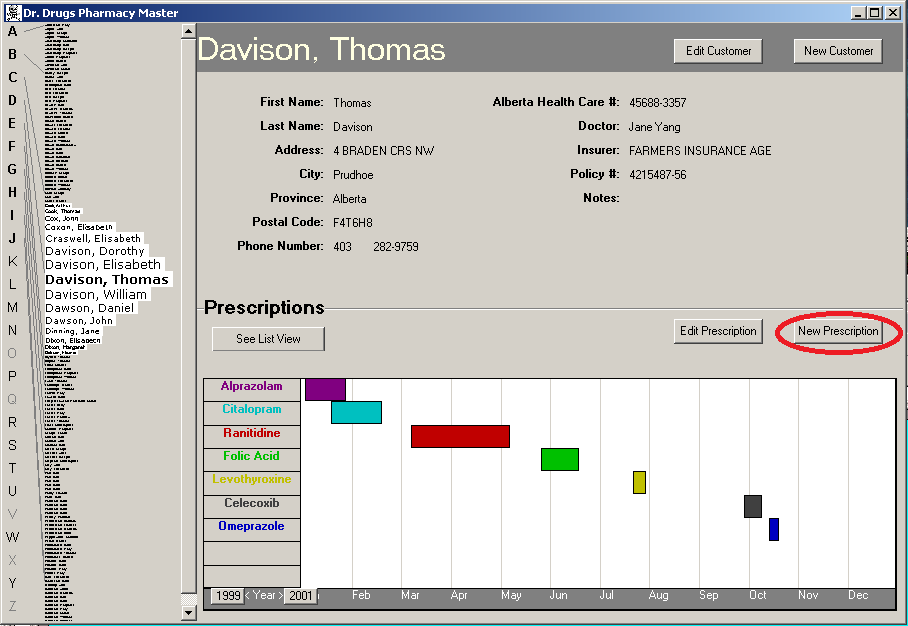
\includegraphics[scale = 0.47]{10_Picture1.png}
  	\end{figure}

    \hspace{150px}\fontsize{7pt}{10pt}\textbf{Good: Information all in the same place}
   
 	\fontsize{4pt}{0.5pt}\selectfont{\color{gray}By previous 481 students Brant LeClercq, Lloyd Yoon, Amy Yang (with permission)}
\end{frame}



%Tica Alexandru
%nr slide 11
\begin{frame}
{\textbf{1. Simple and natural dialogue}}{\textcolor{red}{\rule{12cm}{1.2pt}}}

	\begin{figure}[b]
      
\includegraphics[scale = 0.47]{11_Picture1.png}
  	\end{figure}

    \hspace{150px}\fontsize{7pt}{10pt}\textbf{Good: Stable parts of the window}

   \hspace{150px}\fontsize{7pt}{10pt}\textbf{Bad: Prescriptions separate from graphics}
   
 	\fontsize{4pt}{0.5pt}\selectfont{\color{gray}By previous 481 students Brant LeClercq, Lloyd Yoon, Amy Yang (with permission)}
\end{frame}



%Tica Alexandru
%nr slide 12
\begin{frame}
{\textbf{1. Simple and natural dialogue}}{\textcolor{red}{\rule{12cm}{1.2pt}}}

	\begin{figure}[b]
      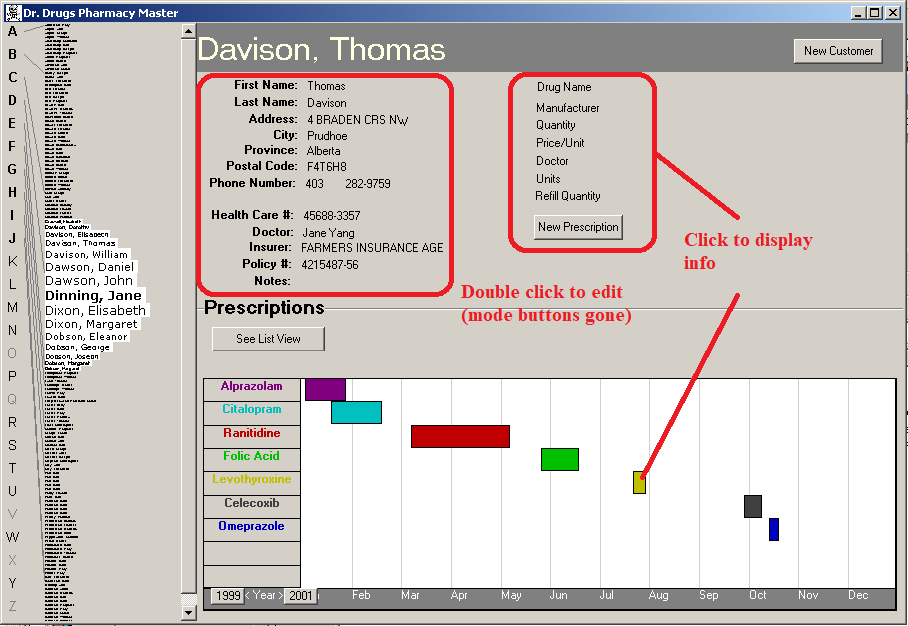
\includegraphics[scale = 0.47]{12_Picture1.png}
  	\end{figure}
   
 	\fontsize{4pt}{0.5pt}\selectfont{\color{gray}By previous 481 students Brant LeClercq, Lloyd Yoon, Amy Yang (with permission)}
\end{frame}



%Tica Alexandru
%nr slide 13
\begin{frame}
{\textbf{2. Speak the users' language}}{\textcolor{red}{\rule{12cm}{1.2pt}}}

\begin{figure}
 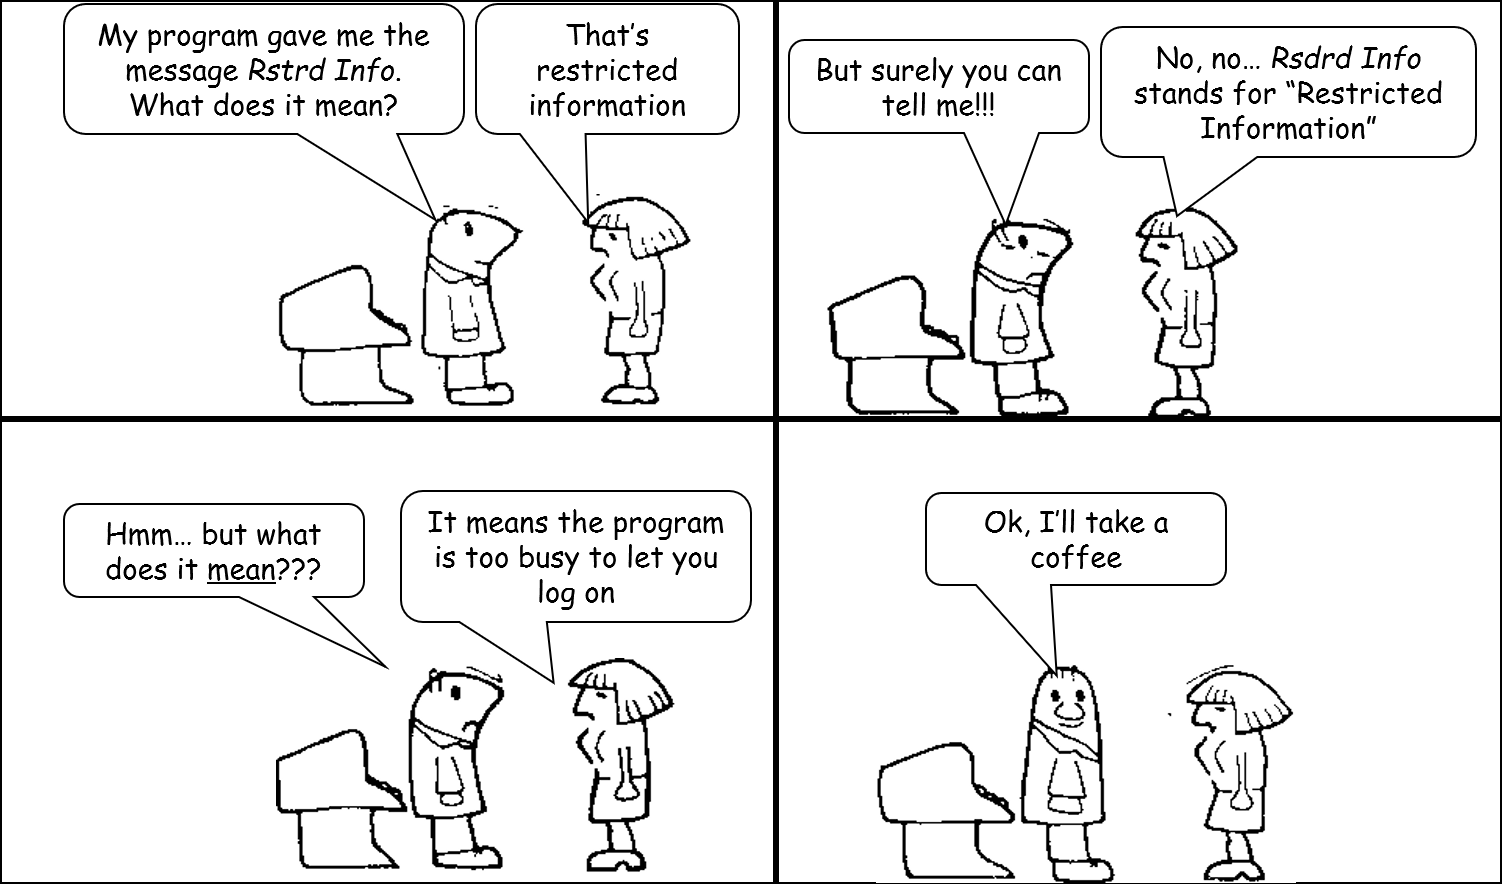
\includegraphics[scale = 0.45]{13_Picture1.png}
\end{figure}

\end{frame}



%Tica Alexandru
%nr slide 14
\begin{frame}
{\textbf{2. Speak the users' language}}{\textcolor{red}{\rule{12cm}{1.2pt}}}

\textbf{Terminology based on users' language for task}
\begin{itemize}
\item [--] e.g. withdrawing money from a bank machine
\end{itemize}

\begin{figure}[H]  
  \begin{minipage}[b]{0.4\linewidth}
    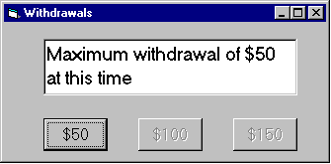
\includegraphics[width=.7\linewidth]{14_Picture1.png}  
  \end{minipage} 
  \begin{minipage}[b]{0.4\linewidth}
    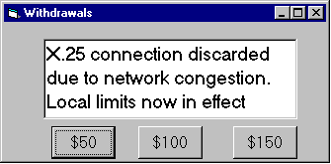
\includegraphics[width=0.7\linewidth]{14_Picture2.png} 
  \end{minipage} 
\end{figure}

\textbf{Use meaningful mnemonics, icons \& abbreviations}

\begin{itemize}
	\item [--]e.g. File / Save
	\begin{itemize}
		\item [$\bullet$]Ctrl + S   \hspace{60px}{(abreviation)}
		\item[$\bullet$]Alt FS  
        \hspace{67px}{(mnemonic for menu action)}
		\item[$\bullet$] 
        %\begin{figure}  
        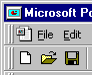
\includegraphics[width=.1\linewidth]{14_Picture3.png} \hspace{67px}{(tooltip  icon)}
        	%\end{figure}
	\end{itemize}
\end{itemize}
\end{frame}



%Tica Alexandru
%nr slide 15
\begin{frame}
{\textbf{2. Speak the users' language}}{\textcolor{red}{\rule{12cm}{1.2pt}}}

\begin{picture}(0,0)
		\put(160,-30){\hbox{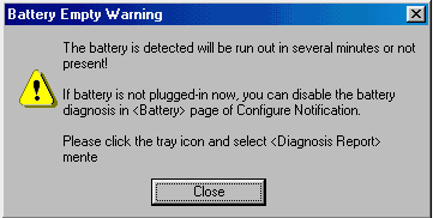
\includegraphics[scale=0.50]{15_Picture1.png}}}
	\end{picture}
	\begin{picture}(0,0)
    	\put(0,-170){\hbox{
\includegraphics[scale=0.45]{15_Picture2.png}}}
	\end{picture}
	\begin{picture}(0,0)
		\put(230,-170){\hbox{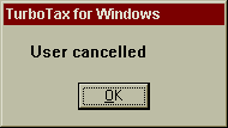
\includegraphics[scale=0.5]{15_Picture3.png}}}
	\end{picture}
    \vspace{100px}

\end{frame}



%Tica Alexandru
%nr slide 16
\begin{frame}
{\textbf{3. Minimize user's memory load}}{\textcolor{red}{\rule{12cm}{1.2pt}}}

\vspace{-70px}
\textbf{Computers good at remembering, people are not!}

\textbf{Promote recognition over recall}

\begin{itemize}
\item [--]menus, icons, choice dialog boxes vs commands, field formats
\item[--]relies on visibility of objects to the user (but less is more!)
\end{itemize}
\vspace{20px}
\begin{picture}(0,0)
		\put(0,-80){\hbox{
\includegraphics[scale=0.50]{16_Picture1.png}}}
	\end{picture}
	\begin{picture}(0,0)
    	\put(135,-100){\hbox{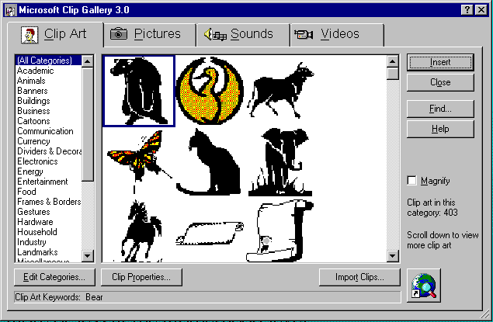
\includegraphics[scale=0.4]{16_Picture2.png}}}
	\end{picture}
\end{frame}



%UNC Roxana Larisa
%Numarul slide-ului: 17
\begin{frame}
{\textbf{3. Minimize user's memory load}}{\textcolor{red}{\rule{12cm}{1.2pt}}}

\bigskip
\bigskip
\bigskip

	\textbf{Give input formats, examples and default values}
     
	\begin{picture}(0,0)
		\put(10,-100){\hbox{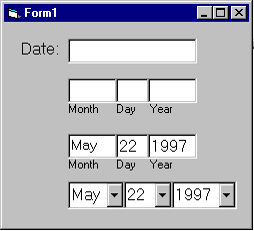
\includegraphics[scale=0.50]{17_picture1.png}}}
	\end{picture}
    \begin{picture}(0,0)
        \put(140,-100){\hbox{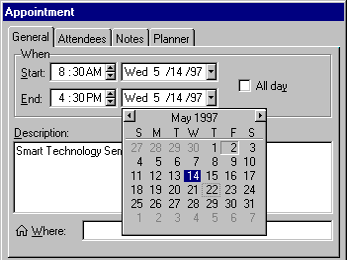
\includegraphics[scale=0.50]{17_picture2.png}}}
    \end{picture}
 
    \vspace{500px}
    
\end{frame} 



%UNC Roxana Larisa
%Numarul slide-ului: 18
\begin{frame}
{\textbf{3. Minimize user's memory load}}{\textcolor{red}{\rule{12cm}{1.2pt}}}

    \textbf{Small number of rules applied universally}
     \begin{itemize}
      \item[--] generic commands
      \begin{itemize}
        	\item[\textcolor{black}{•}] same command can be applied to all 					interface objects
            \begin{itemize}
      			\item[--] interpreted in context of interface object
                \newline
            \end{itemize}
			\item[\textcolor{black}{•}] copy, cut, paste, drag ’n drop, 			... for characters, words, paragraphs, circles, files
               \newline
			\item[\textcolor{black}{•}] context menus
      \end{itemize}
    \end{itemize}
    
\end{frame}



%UNC Roxana Larisa
%Numarul slide-ului: 19
\begin{frame}
{\textbf{3. Minimize user's memory load}}{\textcolor{red}{\rule{12cm}{1.2pt}}}

	\begin{figure}
		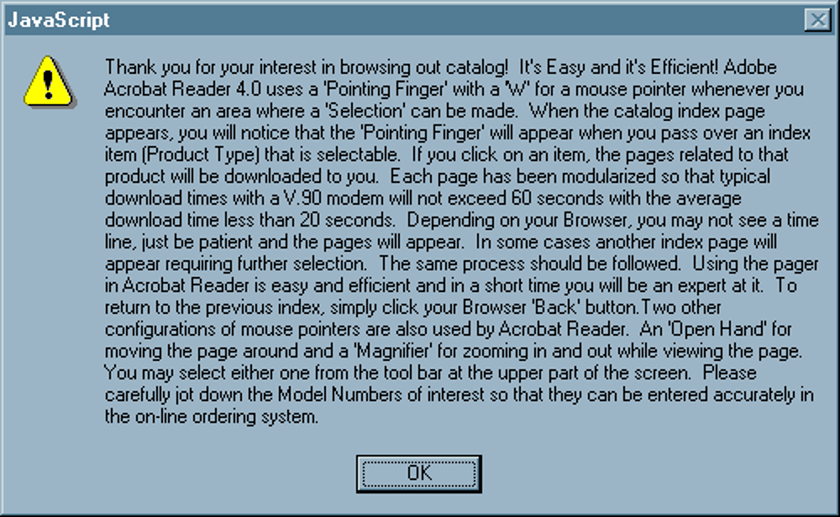
\includegraphics[scale=0.5]{19_picture.png}
  	\end{figure}
    
\end{frame}



%UNC Roxana Larisa
%Numarul slide-ului: 20
\begin{frame}
{\textbf{4. Be consistent}}{\textcolor{red}{\rule{12cm}{1.2pt}}}
	
	\vspace{-5px}\textbf{Consistent syntax of input} 
    \newline
    \newline
    \newline
	\textbf{Consistent language and graphics}
	\begin{itemize}
    	\item[--] same visual appearance across the system (e.g. widgets)
        \item[--] same information/controls in same location on all windows
 	\end{itemize}
	\begin{figure}
		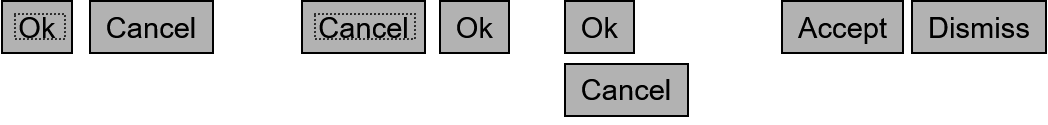
\includegraphics[scale=0.50]{20_picture.png}
  	\end{figure}
    \textbf{Consistent effects}
        \begin{itemize}
    	\item[--] commands, actions have same effect in equivalent situations
			\begin{itemize}
        	\item[\textcolor{black}{•}] predictability
            \end{itemize}
        \end{itemize}
 
\end{frame}


%UNC Roxana Larisa
%Numarul slide-ului: 21
\begin{frame}
{\textbf{4. Be consistent}}{\textcolor{red}{\rule{12cm}{1.2pt}}}

    \begin{picture}(0,0)
    \put(0,20){
	\fbox{\begin{minipage}{13em}
	{\Large{{These are labels with a raised appearance.
	\newline
	\newline
	Is it any surprise that pople try and click on them?}}}
	\end{minipage}\newline}}
    \end{picture}
      
		\begin{picture}(0,0)
			\put(160,-60){\hbox{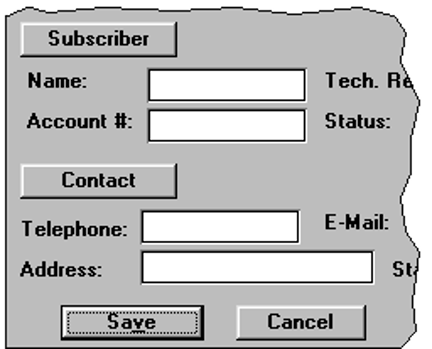
\includegraphics[scale=0.50]{21_picture2.png}}}
          
		\end{picture}
          \begin{tikzpicture}
  			\put(152,60){
  			\draw [black] (0,0) to (-0.5,1) (-0.5,1) to (-1,1);
   }
  \end{tikzpicture}
      
 
\end{frame}



%UNC Roxana Larisa
%Numarul slide-ului: 22
\begin{frame}
{\textbf{4. Be consistent}}{\textcolor{red}{\rule{12cm}{1.2pt}}}

	\begin{figure}
		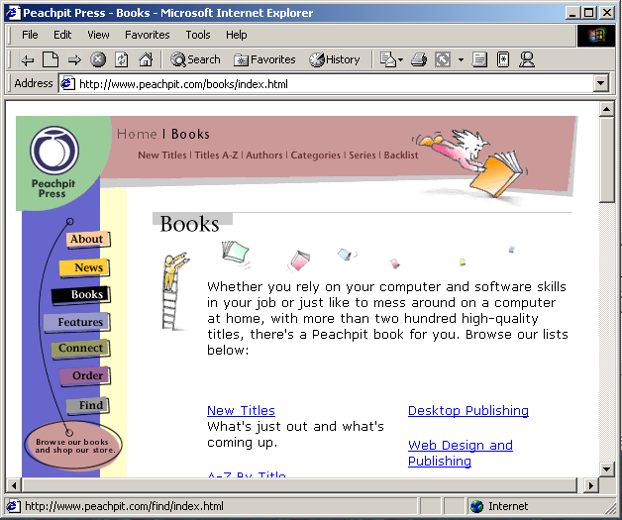
\includegraphics[scale=0.55]{22_picture.png}
  	\end{figure}
\end{frame}



%UNC Roxana Larisa
%Numarul slide-ului: 23
\begin{frame}
{\textbf{4. Be consistent}}{\textcolor{red}{\rule{12cm}{1.2pt}}}

	\begin{figure}
		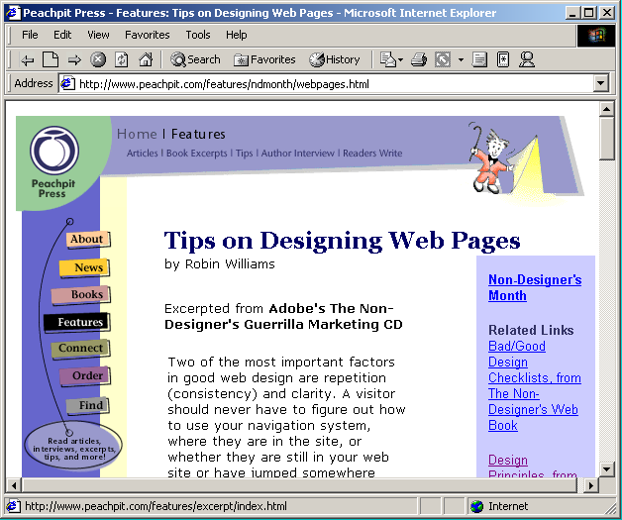
\includegraphics[scale=0.55]{23_picture.png}
  	\end{figure}
\end{frame}



%UNC Roxana Larisa
%Numarul slide-ului: 24
\begin{frame}
{\textbf{5. Provide feedback}}{\textcolor{red}{\rule{12cm}{1.2pt}}}
    
    {Continuously inform the user about:}
	\begin{itemize}
    	\item[--] what it is doing
        \item[--] how it is interpreting the user's input
        \item[--] user should always be aware of what is going on
    
 	\end{itemize}
	
	\begin{picture}(0,0)
		\put(0,80){\hbox{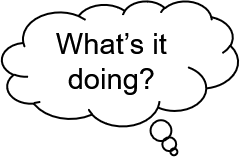
\includegraphics[scale=0.50]{24_picture1.png}}}
	\end{picture}
    \begin{picture}(0,0)
        \put(30,-10){\hbox{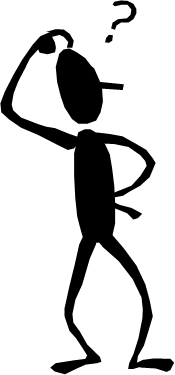
\includegraphics[scale=0.50]{24_picture2.png}}}
    \end{picture}
	\begin{picture}(0,0)
		\put(65,40){\hbox{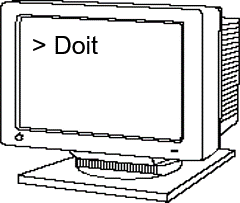
\includegraphics[scale=0.50]{24_picture3.png}}}
	\end{picture}
    \begin{picture}(0,0)
        \put(160,40){\hbox{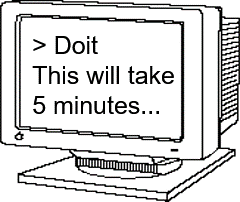
\includegraphics[scale=0.50]{24_picture4.png}}}
    \end{picture}
    	\begin{picture}(0,0)
		\put(210,80){\hbox{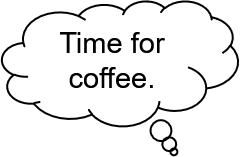
\includegraphics[scale=0.50]{24_picture5.png}}}
	\end{picture}
    \begin{picture}(0,0)
        \put(200,-10){\hbox{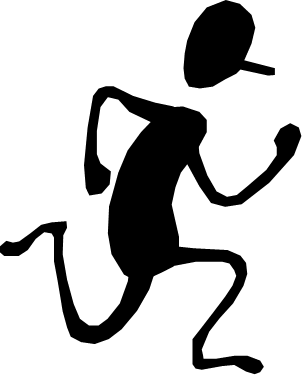
\includegraphics[scale=0.50]{24_picture6.png}}}
    \end{picture}
    \put(130,-10){\textcolor{blue}{\line(0,150){130}}}

\end{frame}



%Vasile Mihai
%numar slide 25
%NOT finished yet
\begin{frame}
{\textbf{5. Provide feedback}}{\textcolor{red}{\rule{12cm}{1.2pt}}}

        \begin{picture}(0,0)
      \put(110,-10){\hbox{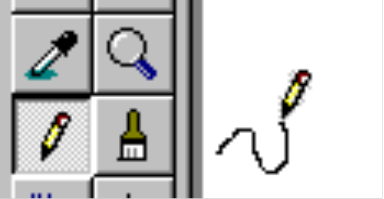
\includegraphics[scale=0.55]{25_picture1.png}}}
  	\end{picture}
            \begin{picture}(0,0)
      \put(5,-75){\hbox{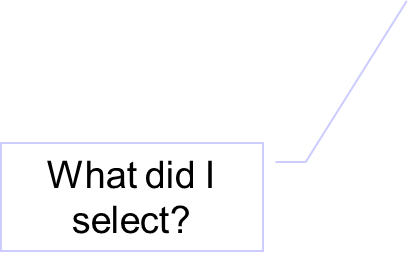
\includegraphics[scale=0.55]{25_picture2.png}}}
  	\end{picture}
            \begin{picture}(0,0)
      \put(185,15){\hbox{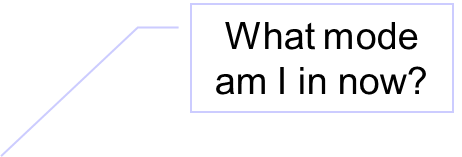
\includegraphics[scale=0.55]{25_picture3.png}}}
  	\end{picture}
            \begin{picture}(0,0)
      \put(175,-110){\hbox{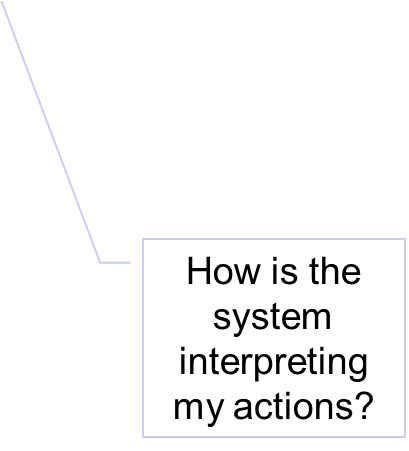
\includegraphics[scale=0.55]{25_picture4.png}}}
  	\end{picture}
\end{frame}



%Vasile Mihai
%numar slide 26
%NOT finished yet
\begin{frame}
{\textbf{5. Provide feedback}}{\textcolor{red}{\rule{12cm}{1.2pt}}}

\text{\Large Be as specific as possible, based on user's input\Large}

\begin{figure}[H]  
  \begin{minipage}[b]{0.4\linewidth}
    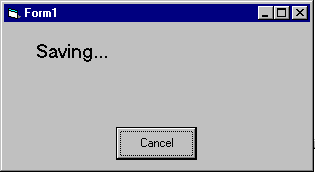
\includegraphics[width=1\linewidth]{26_picture1.png} 
    
  \end{minipage} 
  \begin{minipage}[b]{0.4\linewidth}
    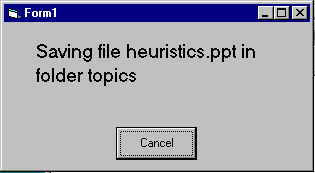
\includegraphics[width=1\linewidth]{26_picture2.png} 
   
  \end{minipage} 
  \end{figure}
  \begin{figure}[H]  
 
  \begin{minipage}[b]{0.5\linewidth}
    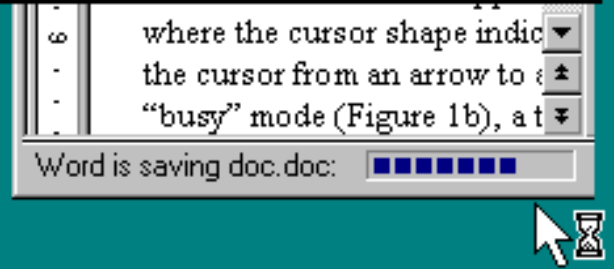
\includegraphics[width=1\linewidth]{26_picture3.png} 
   
  \end{minipage} 
  \end{figure}

\text{\Large Best within the context of the action\Large}

\end{frame}



%Vasile Mihai
%numar slide 28
%NOT finished yet
\begin{frame}
{\textbf{5. Provide feedback}}{\textcolor{red}{\rule{12cm}{1.2pt}}}
    
      \text{\Large Response time\Large}
    \begin{itemize}
    	
        \item[--] how users perceive delays
        \begin{itemize}
        	 \bigskip
        	\item[\textcolor{black}{<0.1s}] perceived as "instantaneous"
             \bigskip
            \item[\textcolor{black}{1s}] user's flow of thought stays uninterrupted, but delay noticed
             \bigskip
             \item[\textcolor{black}{10s}] limit for keeping user's attention focused on the dialog
              \bigskip
              \item[\textcolor{black}{>10s}] user will want to perform other tasks while waiting
        \end{itemize}
    \end{itemize}
 
\end{frame}



%Vasile Mihai
%numar slide 29
%%%%%%%%%%%%%%%%%%%%%%%% de schimbat pozele
\begin{frame}
{\textbf{5. Provide feedback}}{\textcolor{red}{\rule{12cm}{1.2pt}}}

\text{\Large Dealing with long delays\Large}
\bigskip
\bigskip
\begin{itemize}
     \item[\textcolor{black}{--}]Cursors
       \begin{itemize}        	
        	\item[\textcolor{black}{•}] for short transactions               
        \end{itemize}
     \begin{picture}(0,0)
    \put(145,20){\hbox{
\includegraphics[scale=0.5]{29_picture1.png}}}
    \end{picture}
     \item[\textcolor{black}{--}] Percentage progress bars

     \begin{itemize}        	
        	\item[\textcolor{black}{-}] time left       
            \item[\textcolor{black}{-}] estimated time
        \end{itemize}
     \begin{picture}(0,0)
    \put(145,0){\hbox{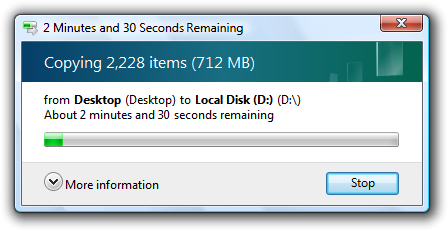
\includegraphics[scale=0.35]{progress-bars-image21.png}}}
    \end{picture}
     \begin{picture}(0,0)
    \put(145,-60){\hbox{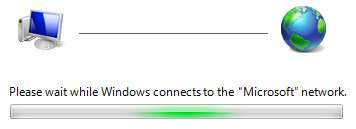
\includegraphics[scale=0.45]{progress-bars-image24.png}}}
    \end{picture}
      \item[\textcolor{black}{--}]Random
        \begin{itemize}        	
        	\item[\textcolor{black}{•}] for unknown times
        \end{itemize}

\end{itemize}

\end{frame}



%Vasile Mihai
%numar slide 30
%NOT finished yet
\begin{frame}
{\textbf{6. Provide clearly marked exits}}{\textcolor{red}{\rule{12cm}{1.2pt}}}

    \begin{picture}(0,0)
      \put(35,-120){\hbox{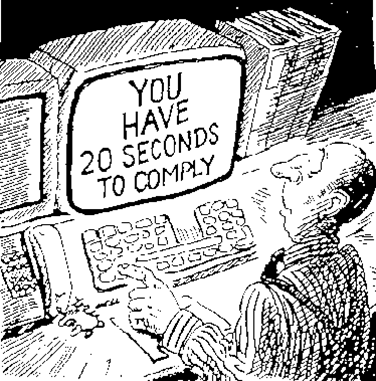
\includegraphics[scale=0.55]{30_picture1.png}}}
  	\end{picture}
        \begin{picture}(0,0)
      \put(240,-10){\hbox{
\includegraphics[scale=0.55]{30_picture2.png}}}
  	\end{picture}

\end{frame}



%Vasile Mihai
%numar slide 31
%NOT finished yet
\begin{frame}
{\textbf{6. Provide clearly marked exits}}{\textcolor{red}{\rule{12cm}{1.2pt}}}

 \text{\Large Users don't like to feel trapped by the computer!\Large
}
    \begin{itemize}
    	
        \item[--] should offer an easy way out of as many situations as possible        
    \end{itemize}
\bigskip
 \text{\Large Strategies:\Large}
	\begin{itemize}
    	\item[--] Cancel button (for dialogues waiting for user input)
        \item[--] Universal Undo (can get back to previous state)
        \item[--] Interrupt (especially for lengthy operations)
        \item[--] Quit (for leaving the program at any time) 
        \item[--] Defaults (for restoring a property sheet)    
 	\end{itemize}
     \begin{picture}(0,0)
      \put(180,-45){\hbox{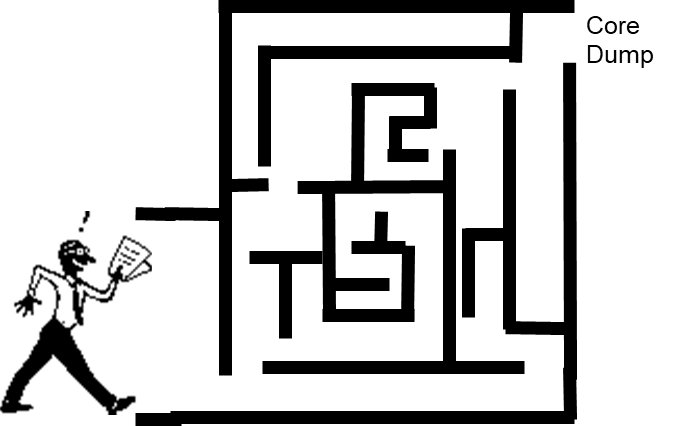
\includegraphics[scale=0.5]{31_picture.png}}}
  	\end{picture}

\end{frame}



%Vasile Mihai
%numar slide 32
%NOT finished yet
\begin{frame}
{\textbf{7. Provide shortcuts}}{\textcolor{red}{\rule{12cm}{1.2pt}}}

    \text{Experienced users - perform frequent operations quickly}
    \bigskip
    \\
          \text{\Large Strategies\Large}
    \begin{itemize}
    	
        \item[--] keyboard and mouse accelerators
        \begin{itemize}        	
        	\item[\textcolor{black}{•}] abbreviations        
            \item[\textcolor{black}{•}] command completion
             \item[\textcolor{black}{•}] context menus
              \item[\textcolor{black}{•}] function keys
              \item[\textcolor{black}{•}] double clicking vs menu selection
        \end{itemize}
        \item[--] type-ahead (entering input before the system is ready for it)
        \item[--] navigation jumps
        \begin{itemize}        	
        	\item[\textcolor{black}{•}] e.g., going to window/location directly, and avoiding intermediate nodes
           
        \end{itemize}
        \item[--] history systems
        \begin{itemize}        	
        	\item[\textcolor{black}{•}] WWW: {\raise.17ex\hbox{$\scriptstyle\mathtt{\sim}$}} 60\% of pages are revisits     
           
        \end{itemize}
    \end{itemize}

\end{frame}



%Zamfir Alexandru
%numar slide 33
\begin{frame}
{\textbf{7. Provide shortcuts}}{\textcolor{red}{\rule{12cm}{1.2pt}}}

\begin{figure}
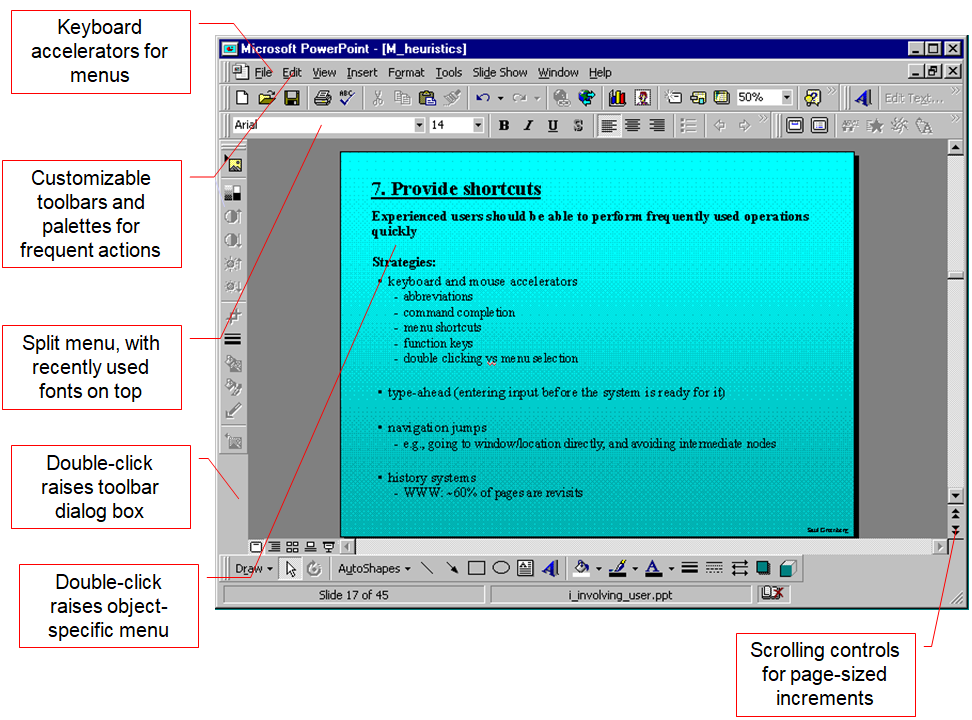
\includegraphics[scale=0.4]{33_picture.png}
\end{figure}

\end{frame}



%Zamfir Alexandru
%numar slide 34
\begin{frame}
{\textbf{7. Provide shortcuts}}{\textcolor{red}{\rule{12cm}{1.2pt}}}

\vspace{-0.5cm}

\begin{figure}
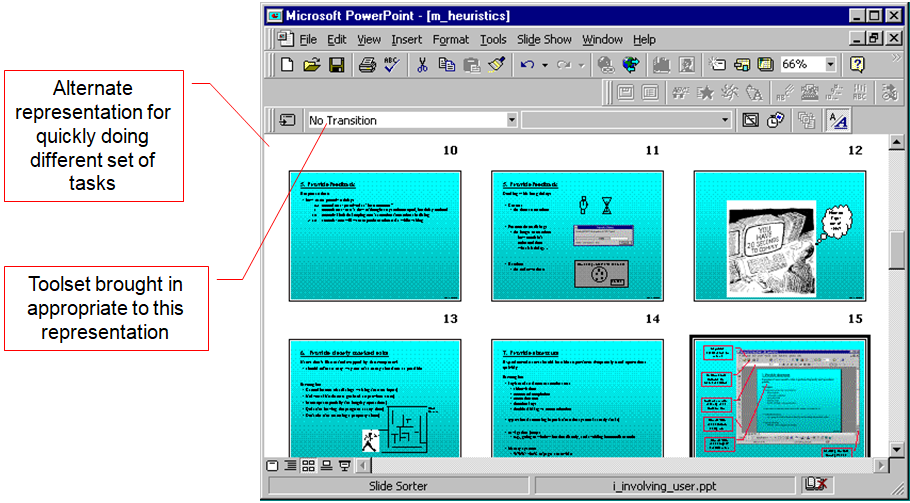
\includegraphics[scale=0.4]{34_picture.png}
\end{figure}

\end{frame}



%Zamfir Alexandru
%numar slide 35
\begin{frame}
{\textbf{8. Deal with errors in a positive manner}}{\textcolor{red}{\rule{12cm}{1.2pt}}}

	\textbf{People will make errors!}\newline\newline
	\bigskip
	\textbf{Errors we make}
	\begin{itemize}
    	\item[--]Mistakes
		\begin{itemize}
        	\item[$\bullet$]conscious deliberations lead to an error instead of correct solution\newline
        \end{itemize}
        \item[--] Slips
        \begin{itemize}
        	\item[$\bullet$]unconscious behaviour gets misdirected en route to satisfying goal
			\begin{itemize}
					\item[--]e.g. drive to store, end up in the office\newline
				\end{itemize}
			\item[$\bullet$]shows up frequently in skilled behaviour
			\begin{itemize}
					\item[--]usually due to inattention\newline
				\end{itemize}
			\item[$\bullet$]often arises from similar actions\newline \newline \newline
        \end{itemize}
	\end{itemize}
\end{frame}



%Zamfir Alexandru
%numar slide 36
\begin{frame}
{\textbf{Designing for slips}}{\textcolor{red}{\rule{12cm}{1.2pt}}}

\large{\textbf{General rules}}
\newline

    \begin{itemize}
		\item[--]prevent slips before they occur
		\item[--]detect and correct slips when they do occur
		\item[--]user correction through feedback and undo \newline\newline\newline\newline\newline\newline\newline\newline\newline     
    \end{itemize}
     \begin{picture}(0,0)
      \put(220,-10){\hbox{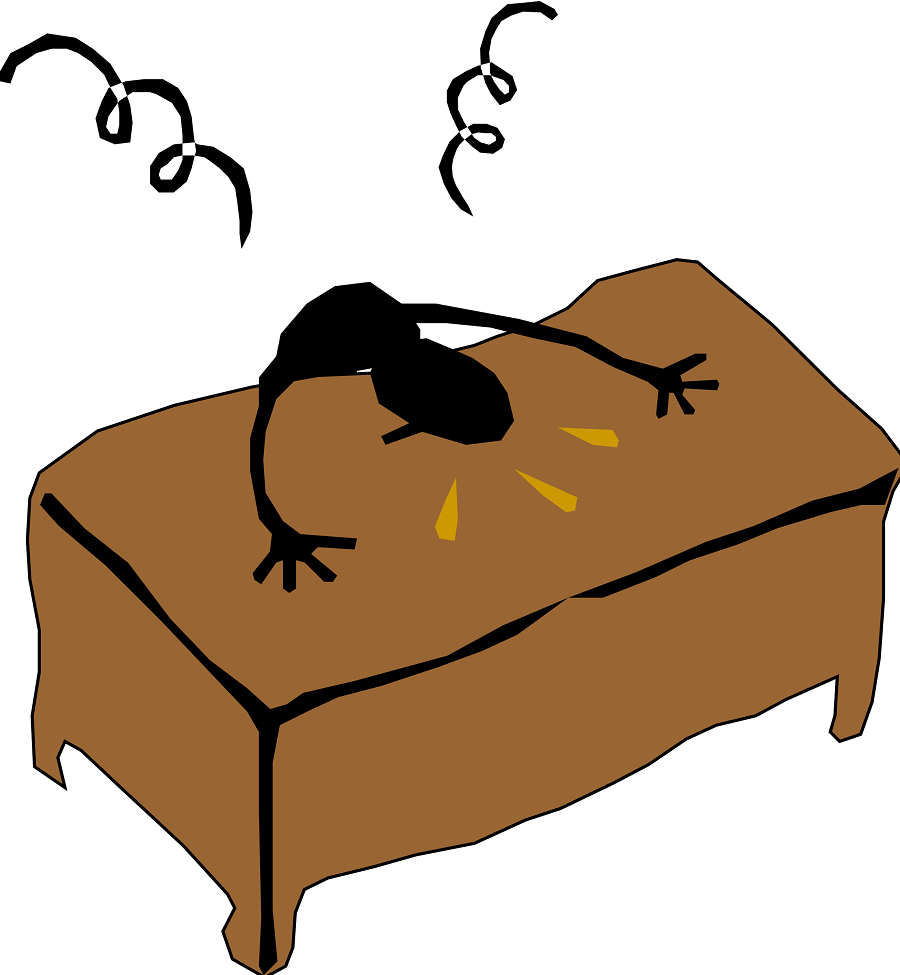
\includegraphics[scale=0.125]{35_picture.png}}}
  	\end{picture}
\end{frame}



%Zamfir Alexandru
%numar slide 37
\begin{frame}
{\textbf{Types of slips}}{\textcolor{red}{\rule{12cm}{1.2pt}}}

	\textbf{Capture error}
	\begin{itemize}
    	\item[--]frequently done activity takes charge instead of one intended
		\item[--]occurs when common \& rarer actions have same initial sequence
		\begin{itemize}
        	\item[$\bullet$]change clothes for dinner and find oneself in bed \tiny{(William James, 1890)}
			\normalsize{\item[$\bullet$]confirm saving of a file when you don’t want to delete it}
        \end{itemize}
        \item[--] minimize by
        \begin{itemize}
        	\item[$\bullet$]make actions undoable instead of confirmation
			\item[$\bullet$]allows reconsideration of action by use
			\begin{itemize}
				\item[--]e.g. open trash to undelete a file\newline \newline \newline \newline \newline
			\end{itemize}
        \end{itemize}
	\end{itemize}
	\begin{picture}(0,0)
      \put(250,0){\hbox{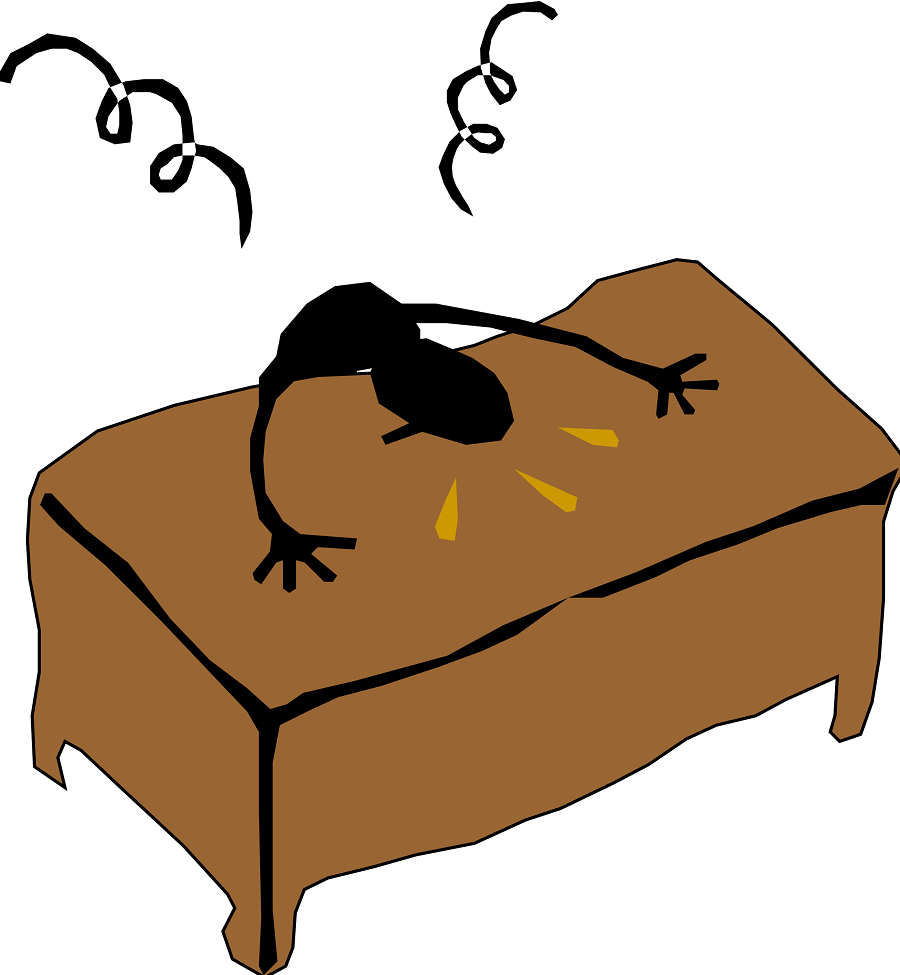
\includegraphics[scale=0.125]{35_picture.png}}}
  	\end{picture}
    \begin{picture}(0,0)
      \put(75,20){\hbox{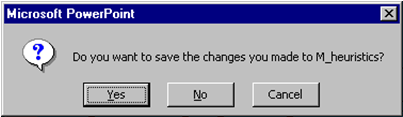
\includegraphics[scale=0.55]{37_picture.png}}}
  	\end{picture}
        \begin{picture}(0,0)
      \put(250,75){\hbox{
\includegraphics[scale=0.25]{37_picture1.png}}}
  	\end{picture}
\end{frame}



%Zamfir Alexandru
%numar slide 38
\begin{frame}
{\textbf{Types of slips}}{\textcolor{red}{\rule{12cm}{1.2pt}}}

	\textbf{Description error}
	\begin{itemize}
    	\item[--]intended action similar to others that are possible
		\begin{itemize}
        	\item[$\bullet$]usually occurs when right \& wrong objects physically near each other
				\begin{itemize}
					\item[--]pour juice into bowl instead of glass 
					\item[--]throw sweaty shirt in toilet instead of laundry basket 
					\item[--]move file to wrong folder with similar name \newline
				\end{itemize}
        \end{itemize}
        \item[--] minimize by
        \begin{itemize}
        	\item[$\bullet$]rich feedback
			\item[$\bullet$]check for reasonable input, etc.
			\item[$\bullet$]undo\newline \newline \newline
        \end{itemize}
	\end{itemize}
	
\end{frame}



%Zamfir Alexandru
%numar slide 39
\begin{frame}
{\textbf{Types of slips}}{\textcolor{red}{\rule{12cm}{1.2pt}}}

	\textbf{Loss of activation}
	\begin{itemize}
    	\item[--] forget what the goal is while undergoing the sequence of actions
		\begin{itemize}
        	\item[$\bullet$]start going to room and forget why you are going there
			\item[$\bullet$]navigating menus/dialogs \& can’t remember what you are looking for
			\item[$\bullet$]but continue action to remember (or go back to beginning)! \newline
        \end{itemize}
        \item[--] minimize by
        \begin{itemize}
        	\item[$\bullet$]if system knows goal, make it explicit
			\item[$\bullet$]if not, allow person to see path taken \newline \newline \newline
        \end{itemize}
	\end{itemize}
	
\end{frame}



%Zamfir Alexandru
%numar slide 40
\begin{frame}
{\textbf{Types of slips}}{\textcolor{red}{\rule{12cm}{1.2pt}}}

	\textbf{Mode errors}
	\begin{itemize}
    	\item[--] people do actions in one mode thinking they are in another
		\begin{itemize}
        	\item[$\bullet$]refer to file that’s in a different directory
			\item[$\bullet$]look for commands / menu options that are not relevant \newline
        \end{itemize}
        
        \item[--] minimize by
        \begin{itemize}
        	\item[$\bullet$]have as few modes as possible (preferably none)
			\item[$\bullet$]make modes highly visible\newline\newline \newline\newline  \newline\newline
        \end{itemize}
	\end{itemize}
	
\end{frame}



%Banuta Mihai Damian
%numar slide 41
\begin{frame}
{\textbf{Generic system responses for errors}}{\textcolor{red}{\rule{12cm}{1.2pt}}}

    \textbf{General idea: Forcing functions }
    \begin{itemize}
    	\item[--] prevent/mitigate continuation of wrongful action
	\end{itemize}
    \textbf{Gag }
    \begin{itemize}
    	\item[--] deals with errors by preventing the user from continuing
    	\begin{itemize}
        	\item[$\bullet$] e.g. cannot get past login screen until correct password entered
      	\end{itemize}
	\end{itemize}
    \textbf{Warn }
    \begin{itemize}
    	\item[--] warn people that an unusual situation is occurring
        \item[--] when overused, becomes an irritant
        \begin{itemize}
        	\item[$\bullet$] e.g.,
        	\begin{itemize}
       			 \item[--] audible bell
        		\item[--] alert box
        	\end{itemize}
        \end{itemize}
	\end{itemize}
 \begin{picture}(0,0)
    \put(130,-5)
	{\hbox{\includegraphics[width=6 cm]{41_Picture1.png}}}
\end{picture} 

\end{frame}



%Banuta Mihai Damian
%numar slide 42
\begin{frame}
{\textbf{Generic system responses for errors}}{\textcolor{red}{\rule{12cm}{1.2pt}}}

\textbf{Do nothing}
\begin{itemize}
\item[--] illegal action just doesn't do anything
\item[--] user must infer what happened

	
		\begin{itemize}
		\item[$\bullet$] enter letter into a numeric-only field (key clicks ignored)

		\item[$\bullet$] put a file icon on top of another file icon (returns it to original position)

		\end{itemize}
	
\end{itemize}

\textbf{Self-correct}
\begin{itemize}
\item[--] system guesses legal action and does it instead
\item[--] but leads to a problem of trust
	\begin{itemize}
		\item[$\bullet$] spelling corrector
		\end{itemize}
	
\end{itemize}

\end{frame}



%Banuta Mihai Damian
%slide 43

\begin{frame}
{\textbf{Generic system responses for errors}}{\textcolor{red}{\rule{12cm}{1.2pt}}}

\textbf{Lets talk about it}
\begin{itemize}
\item[--] system initiates dialog with user to come up with solution to the problem
	\begin{itemize}
		\item[$\bullet$] compile error brings up offending line in source code
		\end{itemize}
\end{itemize}

\textbf{Teach me}
\begin{itemize}
\item[--] system asks user what the action was supposed to have meant
\item[--] action then becomes a legal one
\end{itemize}
\end{frame}



%Banuta Mihai Damian
%slide 44
\begin{frame}
{\textbf{8. Deal with errors in a positive manner}}{\textcolor{red}{\rule{12cm}{1.2pt}}}

\begin{figure}[H]
	\centering
	\includegraphics[width=8cm]{error1.png}
	\center{\textit{What does "0xc0000005" mean?}}
\end{figure}
\end{frame}



%Banuta Mihai Damian 
%slide 45
\begin{frame}
{\textbf{8. Deal with errors in a positive manner}}{\textcolor{red}{\rule{12cm}{1.2pt}}}

\begin{figure}[H]
	\centering
	\includegraphics[width=6cm]{error2.png}
	\center{\textit{Say what?}}
\end{figure}
\end{frame}



%Banuta Mihai Damian 
%slide 46
\begin{frame}
{\textbf{8. Deal with errors in a positive manner}}{\textcolor{red}{\rule{12cm}{1.2pt}}}

\begin{figure}[H]  
	\includegraphics[scale=0.7]{46_Picture4.png} 
	\center{Adobe's \textit{ImageReady}} 
\end{figure}

\begin{figure}[H]  
    \includegraphics[scale=0.7]{46_Picture5.png} 
    \center{\textit{AutoCAD Mechanical} }
\end{figure}

\end{frame}



\begin{frame}
{\textbf{8. Deal with errors in a positive manner}}{\textcolor{red}{\rule{12cm}{1.2pt}}}

\begin{figure}[H]  
    \includegraphics[scale=0.7]{46_Picture6.png} 
    \center{Microsoft Windows' \textit{Notepad}} 
\end{figure}

\begin{figure}[H]  
    \includegraphics[scale=0.7]{46_Picture7.png} 
    \center{Microsoft's \textit{NT Operating System}} 
\end{figure}

\end{frame}



%Banuta Mihai Damian 
%slide 47
\begin{frame}
{\textbf{8. Deal with errors in a positive manner}}{\textcolor{red}{\rule{12cm}{1.2pt}}}

\textbf{Provide meaningful error messages}
\begin{itemize}
		\item[--] error messages should be in the user's task language
		\item[--] don't make people feel stupid
           \begin{itemize}
	         \item[$\break$]Try again, bonehead!
	        
	        \
	        
	        \item[$\break$]Error 25
	        
	        \
	        
	        \item[$\break$]Cannot open this document
	        
	        \
	        
	        \item[$\break$]Cannot open "chapter 5" because the application "Microsoft Word" is not on your system
	        
	        \
	        
	        Cannot open "chapter 5" because the application "Microsoft Word" is not on your system. Open it with "Teachtext" instead?

	    \end{itemize} 
        \end{itemize}
\end{frame}



%Banuta Mihai Damian 
%slide 48
\begin{frame}
{\textbf{8. Deal with errors in a positive manner}}{\textcolor{red}{\rule{12cm}{1.2pt}}}

\textbf{Prevent errors}
\begin{itemize}
\item[--] try to make errors impossible
\item[--] modern widgets:  can only enter legal data
\end{itemize}
\begin{figure}[H]  
  \begin{minipage}[b]{0.4\linewidth}
    \includegraphics[width=.5\linewidth]{48_Picture8.png} 
    
  \end{minipage} 
  \begin{minipage}[b]{0.4\linewidth}
    \includegraphics[width=0.7\linewidth]{48_Picture9.png} 
   
  \end{minipage} 
  \end{figure}

\textbf{Provide reasonableness checks on input data}
\begin{itemize}
\item[--] on entering order for office supplies
	\begin{itemize}
	\item[$\bullet$] 5000 pencils is an unusually large order. Do you really want to order that many?
	\end{itemize}
\end{itemize}
\end{frame}



%Honceriu Tudor
%Numarul slide-ului: 50
\begin{frame}
{\textbf{9. Provide help}}{\textcolor{red}{\rule{12cm}{1.2pt}}}
    
 	\bigskip
    
    \textbf{Help is not a replacement for bad design!}
    \bigskip
   	\begin{wrapfigure}{b}{0.1\textwidth}
      \centering
      \includegraphics[scale = 0.45, right]{50_picture.png}   
	\end{wrapfigure}
    \textbf{Simple systems:}
    \begin{itemize}
      \item[--] {walk up and use}
      \item[--] {minimal instructions}
    \end{itemize}
   	\textbf{Most other systems}
    \begin{itemize}
      \item[--] {feature rich}
	  \item[--] {simple things should be simple}
	  \item[--] {learning path for advanced features}
    \end{itemize}
 	\vspace{40px}
\end{frame}



%Honceriu Tudor
%Numarul slide-ului: 51
\begin{frame}
{\textbf{Documentation and how it is used}}{\textcolor{red}{\rule{12cm}{1.2pt}}}

 	\medskip
 
    \textbf{Many users do not read manuals}
    \begin{itemize}
		\item[--] {prefer to spend their time pursuing their task}
    \end{itemize}
    \medskip
   	\textbf{Usually used when users are in some kind of panic}
    \begin{itemize}
        \item[--] {paper manuals unavailable in many businesses!} 
        \setbeamertemplate{itemize items}[circle]
		\begin{itemize}
      		\item {e.g. single copy locked away in system administrator’s office}
		\end{itemize}
        \item[--] {online documentation better}
        \item[--] {good search/lookup tools}
        \item[--] {online help specific to current context}
    \end{itemize}
    \medskip
    \textbf{Sometimes used for quick reference}
    \begin{itemize}
        \item[--] {syntax of actions, possibilities ...} 
        \item[--] {list of shortcuts ...}
    \end{itemize}
    
\end{frame}



%Honceriu Tudor
%Numarul slide-ului: 52
\begin{frame}
{\textbf{Types of help}}{\textcolor{red}{\rule{12cm}{1.2pt}}}
	
 	\bigskip
  	
	\textbf{Tutorials and/or getting started manuals}
	\begin{itemize}
        \item[--] {short guides that people are likely to read when first obtaining their systems}
		\begin{itemize}
			\item[{•}] {encourages exploration and getting to know the system}
			\item[{•}] {tries to get conceptual material across and essential syntax}
		\end{itemize}
	\medskip
	\item[--] {on-line "tours", exercises, and demos}
	\begin{itemize}
		\item[{•}] {demonstrates very basic principles through working examples}
        \end{itemize}
    \end{itemize}
\end{frame}



%Honceriu Tudor
%Numarul slide-ului: 53
\begin{frame}
{\textbf{Types of help}}{\textcolor{red}{\rule{12cm}{1.2pt}}}

 	\bigskip

	\textbf{Reference manuals} 
	\begin{itemize}
		\item[--] {used mostly for detailed lookup by experts}
		\begin{itemize}
			\item[{•}] {rarely introduces concepts}
			\item[{•}] {thematically arranged}
		\end{itemize}
		\item[--] {on-line hypertext}
		\begin{itemize}
			\item[{•}] {search / find}            
			\item[{•}] {table of contents}
			\item[{•}] {index}
			\item[{•}] {cross-index}    
		\end{itemize}
	\end{itemize}
	\begin{picture}(0,0)
		\put(40,-80){\hbox{\includegraphics[scale=0.50]{53_picture3.png}}}
	\end{picture}
	\begin{picture}(0,0)
    	\put(130,-80){\hbox{\includegraphics[scale=0.45]{53_picture2.png}}}
	\end{picture}
	\begin{picture}(0,0)
		\put(190,-40){\hbox{\includegraphics[scale=0.45]{53_picture1.png}}}
	\end{picture}
    \vspace{100px}
\end{frame}



%Honceriu Tudor
%Numarul slide-ului: 54
\begin{frame}
{\textbf{Types of help}}{\textcolor{red}{\rule{12cm}{1.2pt}}}
	
 	\bigskip

  	\textbf{Reminders}
	\begin{itemize}
		\item[--] {short reference cards}
		\begin{itemize}
        	\item[{•}] {expert user who just wants to check facts}
			\item[{•}] {novice who wants to get overview of system’s capabilities}
        \end{itemize}
		\medskip
		\item[--] {keyboard templates}
      	\begin{itemize}
        	\item[{•}] {shortcuts/syntactic meanings of keys}
        	\item[{•}] {recognition vs. recall}
        	\item[{•}] {capabilities}
        \end{itemize}
        \medskip
		\item[--] {tooltips and other context-sensitive help}
      	\begin{itemize}
        	\item[{•}] {text over graphical items indicates their meaning or purpose}
        \end{itemize}
    \end{itemize}
    \begin{figure}[b]
    	\includegraphics[scale = 0.5, right]{54_picture.png}
    \end{figure}
    \vspace{10px}\hspace{-24px}\fontsize{8pt}{1pt}\selectfont{\color{gray}{Microsoft Word}} 
    
\end{frame}



%Honceriu Tudor
%Numarul slide-ului: 55
\begin{frame}
{\textbf{Types of help}}{\textcolor{red}{\rule{12cm}{1.2pt}}}
  	    
  	\textbf{Wizards}
     \begin{itemize}
      \item[--] {walks user through typical tasks}
      \item[--] {\textit{but} dangerous if user gets stuck}
    \end{itemize}
    
    \medskip

	\begin{picture}(0,0)
		\put(5,-45){\hbox{\includegraphics[scale=0.38]{55_picture1.png}}}
	\end{picture}
    \begin{picture}(0,0)
        \put(50,-120){\hbox{\includegraphics[scale=0.45]{55_picture2.png}}}
    \end{picture}
    \begin{picture}(0,0)
        \put(95,-120){\hbox{\includegraphics[scale=0.57]{55_picture3.png}}}
    \end{picture}
    \vspace{100px}
\end{frame}



%Honceriu Tudor
%Numarul slide-ului: 56
\begin{frame}
{\textbf{Types of help}}{\textcolor{red}{\rule{12cm}{1.2pt}}}
  	
  	\textbf{Tips}
	\begin{itemize}
		\item[--] {migration path to learning system features}
		\item[--] {also context-specific tips on being more efficient}
		\item[--] {must be "smart", otherwise boring and tedious}
    \end{itemize}
    
    \begin{picture}(0,0)
		\put(10,-45){\hbox{\includegraphics[scale=0.50]{56_picture1.png}}}
	\end{picture}
    \begin{picture}(0,0)
        \put(10,-120){\hbox{\includegraphics[scale=0.55]{56_picture2.png}}}
    \end{picture}
    \begin{picture}(0,0)
        \put(40,-90){\hbox{\includegraphics[scale=0.57]{56_picture3.png}}}
    \end{picture}
    \vspace{100px}
\end{frame}



%Paraschiv Marian
%Numarul slide-ului 61
\begin{frame}
{\textbf{Evaluating Heuristic evaluation}}{\textcolor{red}{\rule{12cm}{1.2pt}}}
   
	\begin{itemize}
		\item[] {Problems found by a single inspector}
        \item[] {Problems found by multiple inspectors}
        \item[] {Individuals vs. teams}
        \item[] {Self guided or scenarios?}
    \end{itemize}
\end{frame}



%Paraschiv Marian
%Numarul slide-ului 62
%62_picture.png

\begin{frame}
{\textbf{Problems found by a single inspector}}{\textcolor{red}{\rule{12cm}{1.2pt}}}
   
  	\textbf{Average over six case studies}
	\begin{itemize}
		\item[--] {35\% of all usability problems}
        \item[--] {42\% of the major problems}
        \item[--] {32\% of the minor problems}
    \end{itemize}
    
    \vspace{90px}
    \textbf{Not great, but}
	\begin{itemize}
		\item[--] {finding some problems with one evaluator is \\ \textit{much} better than finding no problems with \\ no evaluators!
}
	\begin{picture}(0,0)
        	\put(130,-5){\hbox{\includegraphics[scale=0.60]{62_picture.png}}}
        \end{picture}
    \end{itemize}
\end{frame}



%Paraschiv Marian
%Numarul slide-ului 63
%62_picture.png
\begin{frame}
{\textbf{Problems found by a single inspector}}{\textcolor{red}{\rule{12cm}{1.2pt}}}

  	\textbf{Varies according to }
	\begin{itemize}
		\item[--] {difficulty of the interface being evaluated }
        \item[--] {the expertise of the inspectors }
    \end{itemize}
    \medskip
    \textbf{Average problems found by:}
	\begin{itemize}
		\item[--] {novice evaluators - 22\%}
        \begin{itemize}
        	\item[{•}] {no usability expertise}
        \end{itemize}
        \item[--] {regular specialists - 41\%}
        \begin{itemize}
        	\item[{•}] {expertise in usability }
        \end{itemize}
       	\item[--] {double specialists  - 60\%}
        \begin{itemize}
        	\item[{•}] {experience in both usability and the\\ particular kind of interface being evaluated }
            \item[{•}] {also find domain-related problems}
        \end{itemize}
	\end{itemize}
    
    \medskip
     \textbf{Tradeoff}
	\begin{itemize}
		\item[--] {novices poorer, but cheaper!}
	\begin{picture}(0,0)
        	\put(75,-5){\hbox{\includegraphics[scale=0.60]{62_picture.png}}}
        \end{picture}
    \end{itemize}
    
\end{frame}



%Paraschiv Marian
%Numarul slide-ului 64
%64_picture.png
\begin{frame}
{\textbf{Problems found by a single inspector}}{\textcolor{red}{\rule{12cm}{1.2pt}}}

    \textbf{Evaluators miss both easy and hard problems}
    	\begin{itemize}
    		\item [--]  {"best" evaluators can miss easy problems}
        	\item [--]  {"worse" evaluators can discover hard problems}
             
    	\end{itemize}
        \begin{picture}(0,0)
        	\put(25,-155){\hbox{\includegraphics[scale=0.50]{64_picture.png}}}
        \end{picture}
    
    \vspace{150px}
\end{frame}



%Stratulat Adrian
%Numarul slide-ului: 65
%65_picture1.png
\begin{frame}
{\textbf{Problems found by multiple inspectors}}{\textcolor{red}{\rule{12cm}{1.2pt}}}

    \textbf{3-5 evaluators find 66-75\% of usability problems}
    	\begin{itemize}
    		\item [--] different people find different usability problems
        	\item [--] only modest overlap between the sets of problems found
    	\end{itemize}
       
        \begin{picture}(0,0)
        	\put(25,-135){\hbox{\includegraphics[scale=0.60]{65_picture1.png}}}
        \end{picture}
    
    \vspace{150px}
\end{frame}



%Stratulat Adrian
%Numarul slide-ului: 66
%66_picture1.png
\begin{frame}
{\textbf{Problems found by multiple inspectors}}{\textcolor{red}{\rule{12cm}{1.2pt}}}

    \textbf{Where is the best cost/benefit?}
    
    \begin{picture}(0,0)
    	\put(20,-160){\hbox{\includegraphics[scale=0.60]{66_picture1.png}}}
    \end{picture}
    
    \vspace{180px}
\end{frame}



%Stratulat Adrian
%Numarul slide-ului: 67
%67_picture1.png
\begin{frame}
{\textbf{Individuals \textit{vs} teams}}{\textcolor{red}{\rule{12cm}{1.2pt}}}

    \textbf{Nielsen}
    \begin{itemize}
    	\item [--] recommends individual evaluators inspect the interface alone
    \end{itemize}
    \bigskip
    \textbf{Why?}
    \begin{itemize}
    	\item [--] evaluation is not influenced by others
        \item [--] independent and unbiased
        \item [--] greater variability in the kinds of errors found
        \item [--] no overhead required to organize group meetings
    \end{itemize}
    
    \begin{picture}(0,0)
    	\put(220,-70){\hbox{\includegraphics[scale=0.50]{67_picture1.png}}}
    \end{picture}
    
    \vspace{70px}
\end{frame}



%Stratulat Adrian
%Numarul slide-ului: 68
\begin{frame}
{\textbf{Self Guided \textit{vs} Scenario Exploration}}{\textcolor{red}{\rule{12cm}{1.2pt}}}

    \textbf{Self-guided}
    \begin{itemize}
    	\item [--] open-ended exploration
        \item [--] not necessarily task-directed
        \item [--] good for exploring diverse aspects of the interface, and to follow potential pitfalls
    \end{itemize}
    \bigskip
    \textbf{Scenarios}
    \begin{itemize}
    	\item [--] step through the interface using representative end user tasks
        \item [--] ensures problems identified in relevant portions of the interface
        \item [--] ensures that specific features of interest are evaluated
        \item [--] but limits the scope of the evaluation - problems can be missed
    \end{itemize}
    
    \vspace{30px}
\end{frame}



\begin{frame}
{\textbf{Other guidelines}}{\textcolor{red}{\rule{12cm}{1.2pt}}}
   
	\begin{itemize}
		\item[] {Style guides}
    \end{itemize}
\end{frame}



%Paraschiv Marian
%Numarul slide-ului 57
\begin{frame}
{\textbf{Style guides}}{\textcolor{red}{\rule{12cm}{1.2pt}}}
   
  	\textbf{Guidelines published by producers of graphical user interfaces (GUIs)}
	\begin{itemize}
		\item[--] {example}
		\begin{itemize}
            \item[{•}] {Microsoft Windows}
            \item[{•}] {Apple}
            \item[{•}] all major software platforms have published guidelines for user interface design
        \end{itemize}
    \end{itemize}

    \textbf{Describes the "look and feel" of the GUI}

    \textbf{Good, but hard too follow}
	\begin{itemize}
		\item[--] {GUI and widget specific}
		\item[--] {vast number of guidelines}
        \item[--] {may miss fundamental design principles}
    \end{itemize}
\end{frame}



\begin{frame}
{\textbf{Style guides}}{\textcolor{red}{\rule{12cm}{1.2pt}}}
   
  	\textbf{Microsoft Windows}
	\begin{itemize}
		\item[--] User experience guidelines for Windows-based desktop applications
		
		\url{https://docs.microsoft.com/en-us/windows/desktop/uxguide/guidelines}

		\item[--] User Interface Principles
				
		\url{https://docs.microsoft.com/en-us/windows/desktop/appuistart/-user-interface-principles}
    \end{itemize}

\end{frame}



\begin{frame}
{\textbf{Style guides}}{\textcolor{red}{\rule{12cm}{1.2pt}}}

  	\textbf{Apple}
	\begin{itemize}
		\item[--] Human Interface Guidelines

		\url{https://developer.apple.com/design/human-interface-guidelines/}
				
    \end{itemize}
       
  	\textbf{Android}
	\begin{itemize}
		\item[--] Android Design Guidelines
		
		\url{https://developer.android.com/design}
    \end{itemize}

\end{frame}



%Paraschiv Marian
%Numarul slide-ului 60
\begin{frame}
{\textbf{You know now}}{\textcolor{red}{\rule{12cm}{1.2pt}}}

  	\textbf{Nine principles of design}
	\begin{itemize}
		\item[--] {Simple and natural dialogue}
        \item[--] {Speak the user's language}
        \item[--] {Minimize user's memory load}
        \item[--] {Be consistent}
        \item[--] {Provide feedback}
        \item[--] {Provide clearly marked exits}
        \item[--] {Provide shortcuts}
        \item[--] {Deal with errors in a positive manner}
        \item[--] {Provide help}
    \end{itemize}

    \textbf{Heuristic evaluation}
	\begin{itemize}
		\item[--] {Principles can be used to systematically inspect the interface for usability problems}
    \end{itemize}

    \textbf{Style guides}
\end{frame}



\usetikzlibrary{arrows,positioning} 
\tikzset{
    %Define style for boxes
    punkt/.style={
           rectangle,
           draw=blue, thick,
           minimum height=2em,
           text centered},
    dreptunghi/.style={
           rectangle,
           draw=black,
           minimum height=2em}
}

\newcommand{\sageatainsus}[7]{

\begin{tikzpicture}
        \node [single arrow,minimum width=#1, minimum height=#2,draw=black, rotate=#7,line width=#5,inner sep=#3] {   };
        \coordinate (P) at (0,0);
        \node[text width=#4] (N) at (P) {#6} ;
		
\end{tikzpicture}

}


%$ lungime text, grosime dreptunghi, text
\newcommand{\dreptunghi}[3]{

\begin{tikzpicture}
\node[dreptunghi,text width=#1,line width=#2] {#3};
\end{tikzpicture}

}
% culoare, grosime, lungime
\newcommand{\linie}[3]{
\begin{tikzpicture}
\draw[draw=#1,line width=#2] (0,0) -- (0,-#3) ;
\end{tikzpicture}
}


%spatiul intre linii
\renewcommand{\baselinestretch}{0.5} 

%Raceanu Dragos
%Numarul slide-ului:49
\begin{frame}
{\textbf{Interface Design and Usability Engineering}}{\textcolor{red}{\rule{12cm}{1.2pt}}}

\vspace{-48px}


 \begin{picture}(0,0)
        \put(26,-265){\hbox{\includegraphics[scale=0.53]{99_picture.png}}}
 \end{picture}
 
  %%sagetile lipsa
\begin{picture}(0,0)
\put(118,-242){
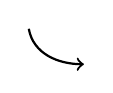
\begin{tikzpicture}
\draw [->,black,line width=0.8] (0,0) to [out=-80,in=180] (0.7,-0.45);
\end{tikzpicture}}
\put(118,-188){
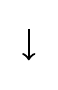
\begin{tikzpicture}
\draw [->,black,line width=0.8] (0,0) to (0,-0.4);
\end{tikzpicture}}

\put(212,-244){
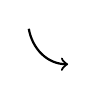
\begin{tikzpicture}
\draw [->,black,line width=0.8] (0,0) to [out=-80,in=180] (0.5,-0.45);
\end{tikzpicture}}
\put(206,-188){
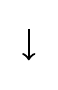
\begin{tikzpicture}
\draw [->,black,line width=0.8] (0,0) to (0,-0.4);
\end{tikzpicture}}
\end{picture}


% culoare, grosime, plecare (cu minus),lungime

\begin{picture}(0,0)
\put(90,-260){\linie{gray}{3}{8.5}}
\end{picture}


\begin{picture}(0,0)
\put(185,-247){\linie{gray}{3}{8.5}}
\end{picture}

\begin{picture}(0,0)
\put(270,-232){\linie{gray}{3}{8.5}}
\end{picture}

\vspace{-11px}


%%sus

\hspace{-29px}\textit{\textbf{\fontsize{9pt}{0pt}\selectfont{\color{black}Goals:
}}}

%dreaptunghiul 1
\begin{picture}(0,0)
\put(20,0)
{\dreptunghi{1.7cm}{0.6}{
\textbf{\fontsize{6pt}{0pt}\selectfont{\color{black}Articulate:\\
\textbullet who users are \\
\textbullet their key tasks
}}}}
\end{picture}



%dreptughiul 2
\begin{picture}(0,0)
\put(122,15)
{\dreptunghi{1.2cm}{0.6}{
\textbf{\fontsize{6pt}{0pt}\selectfont{\color{black}Brainstorm designs
}}}}
\end{picture}

%dreptughiul 3
\begin{picture}(0,0)
\put(212,30)
{\dreptunghi{1.2cm}{0.2}{
\textbf{\fontsize{6pt}{0pt}\selectfont{\color{black}Refined designs
}}}}
\end{picture}

%dreptughiul 4
\begin{picture}(0,0)
\put(285,42)
{\dreptunghi{1.1cm}{0.2}{
\textbf{\fontsize{6pt}{0pt}\selectfont{\color{gray}Completed designs
}}}}
\end{picture}


\vspace{30px}


%mij

\hspace{-29px}\textit{\textbf{\fontsize{8.5pt}{0pt}\selectfont{\color{black}Methods:
}}}

%sageata 1
\vspace{20px}
 \begin{picture}(0,0)
 \put(-4,-12){\sageatainsus{5.5em}{7.4em}{4mm}{1.25cm}{0.4}{\fontsize{6pt}{1pt}\selectfont{\color{black}Task centered system \vspace{4px} design 
Participatory  \vspace{4px} design
User-centered design}}{-90}}
 \end{picture}

%sageata 2
 \begin{picture}(0,0)
\put(47,7){\sageatainsus{1.8em}{6.8em}{4.5mm}{0.9cm}{0.6}{\fontsize{6pt}{0pt}\selectfont{\color{black} Evaluate tasks}}{90}}
 \end{picture}


%sageata 3
\begin{picture}(0,0)
\put(90,18){\sageatainsus{5em}{7em}{5mm}{1.3cm}{0.4}{
\textbf{\fontsize{6pt}{0pt}\selectfont{\color{black} Psychology of everyday \vspace{4px}  things}}

\fontsize{6pt}{0pt}\selectfont{\color{black} User \vspace{4px} involvement}

\textbf{\fontsize{6pt}{0pt}\selectfont{\color{black} Representation \& metaphors}}
}{-90}}
 \end{picture}
 
 
 %sageata 3 jos
\begin{picture}(0,0)
\put(90,-20){\sageatainsus{5em}{0em}{5mm}{1.2cm}{0.4}{
\textbf{\fontsize{6pt}{0pt}\selectfont{\color{black} low fidelity prototyping methods}}

}{-90}}
 \end{picture}
 
%sageata 4
\begin{picture}(0,0)
\put(137,50){\sageatainsus{4.5em}{7.4em}{5mm}{1.2cm}{0.4}{

\textit{\fontsize{6pt}{0pt}\selectfont{\color{black} Participatory \vspace{8px} interaction}}

\textit{\fontsize{6pt}{0pt}\selectfont{\color{black} Task scenario walk-through
}}

}{90}}
 \end{picture}

%sageata 5
\begin{picture}(0,0)
\put(185,60){\sageatainsus{4em}{7em}{5mm}{1cm}{0.4}{

\fontsize{6pt}{0pt}\selectfont{\color{black}Graphical screen  \vspace{4px} design}

\fontsize{6pt}{0pt}\selectfont{\color{red}Interface \vspace{4px} guidelines}

\fontsize{6pt}{0pt}\selectfont{\color{red}Style  \vspace{4px} guides}

}{-90}}
 \end{picture}
 
 
 %sageata 5 jos
\begin{picture}(0,0)
\put(185,20){\sageatainsus{5em}{4em}{5mm}{1.2cm}{0.4}{
\textbf{\fontsize{6pt}{0pt}\selectfont{\color{black} high fidelity prototyping methods}}

}{-90}}
 \end{picture}

%sageata 6
\begin{picture}(0,0)
\put(228,88){\sageatainsus{4em}{7em}{5mm}{1cm}{0.4}{

\textit{\fontsize{6pt}{0pt}\selectfont{\color{black} Usability
 \vspace{8px} testing}}

\textit{\fontsize{6pt}{0pt}\selectfont{\color{red} Heuristic evaluation}}
}{90}}
 \end{picture}

%sageata 7
\begin{picture}(0,0)
\put(296,103){\sageatainsus{2.5em}{7em}{3.6mm}{0.7cm}{0.4}{

\textit{\fontsize{6pt}{0pt}\selectfont{\color{gray}Field testing}}
}{90}}
 \end{picture}
 
 
 
 \vspace{-39px}
 %%jos

\hspace{-29px}\vspace{25px}\textit{\textbf{\fontsize{9pt}{0pt}\selectfont{\color{black}Products:
}}}

%dreptunghiul 1
\begin{picture}(0,0)
\put(20,27)
{\dreptunghi{1.4cm}{0.2}{
\textbf{\fontsize{6pt}{0pt}\selectfont{\color{black}User and task descriptions
}}}}
\end{picture}

%dreptunghiul 2
\begin{picture}(0,0)
\put(120,40)
{\dreptunghi{1.4cm}{0.2}{
\textbf{\fontsize{6pt}{0pt}\selectfont{\color{black}Throw-away paper prototypes
}}}}
\end{picture}

%dreptunghiul 3
\begin{picture}(0,0)
\put(205,56)
{\dreptunghi{1.2cm}{0.2}{
\textbf{\fontsize{6pt}{0pt}\selectfont{\color{black}Testable prototypes
}}}}
\end{picture}

%dreptunghiul 4
\begin{picture}(0,0)
\put(280,60)
{\dreptunghi{1.4cm}{0.2}{
\textbf{\fontsize{6pt}{0pt}\selectfont{\color{gray}Alpha/beta systems or complete specification
}}}}
\end{picture}

\end{frame}



{\setbeamercolor{background canvas}{bg=background}
\begin{frame}
{\textbf{*Bibliography}}{\textcolor{red}{\rule{12cm}{1.2pt}}}

        \begin{itemize}
        	\item[{$\bullet$}] Saul Greenberg, \textbf{Principles for Design. Design guidelines and usability heuristics}, University of Calgary, Canada

        	\url{http://pages.cpsc.ucalgary.ca/~saul/481/}
			\newline

			\item[{$\bullet$}] Keith Andrews, \textbf{Human Computer Interaction, Chapter 8. Usability Inspection Methods}, TU Graz, Austria

        	\url{https://courses.isds.tugraz.at/hci/hci.pdf}                			\newline
        	 
     	\end{itemize}
\end{frame}



\end{document}